\chapter{Selective Retransmit}

Assume client device that playsback a video stream. Structurelly, a video is
composed of frames, frames are then segmented into packets to stream across a 
network. The client device recombines the packets into a frame, then sequence
the frame to playback the video.\newline

However, network is not-deterministic. Depending on the route the packets take
to get to the client, they may arrive out-of-order. The client may need to
maintain a receive buffer for the packets, re-order the packets back into
sequence before pushing the packets down to decoding engine.\newline

The network may also drop packets if any of the switches gets too busy. In the
case of a packet drop, the client has a few options. The client can either
discard the frame and let the decoding engine downstream to deal with it (which
may ressult in  visible artifacts during play back). The client can request the
whole frame to be re-sent, which results in additional bandwidith consumption.
The client can selectively request the missing packet to be retransmited, which
will minimize additional bandwidth consumption, but increases implementation 
complexity.\newline 

In this chapter, we will implement a simple selective retransmit
algorithm.\newline

\begin{center}

\begin{tikzpicture}[
    packet/.style={rectangle, draw, fill=blue!20, minimum width=1cm, minimum height=0.8cm},
    missing/.style={rectangle, draw, dashed, fill=red!20, minimum width=1cm, minimum height=0.8cm},
    arrow/.style={->, >=stealth, thick}
]

    % Draw packets
    \node[packet] (p0) at (0,0) {\(pkt\ 0\)};
    \node[packet, right=0.5cm of p0] (p2) {\(pkt\ 1\)};
    \node[missing, right=0.5cm of p2] (missing1) {\(lost\)};
    \node[packet, right=0.5cm of missing1] (p4) {\(pkt\ 3\)};
    \node[packet, right=0.5cm of p4] (p5) {\(pkt\ 4\)};
    \node[right=0.5cm of p5] (dots) {\(\dots\)}; % Just dots, no box
    \node[packet, right=0.5cm of dots] (pn) {\(pkt\_n\)};

    % Draw arrows between packets
    \draw[arrow] (p0.east) -- (p2.west);
    \draw[arrow] (p2.east) -- (missing1.west);
    \draw[arrow] (missing1.east) -- (p4.west);
    \draw[arrow] (p4.east) -- (p5.west);
    \draw[arrow] (p5.east) -- (dots);
    \draw[arrow] (dots) -- (pn.west);

    % Add arrow pointing to "lost" with caption
    \draw[arrow, red] ([yshift=0.3cm] missing1.north) -- (missing1.north) 
        node[midway, above, text=red] {request to retransmit};

\end{tikzpicture}

\end{center}

\section{Requirement}

Since packets may arrive out-of-order, the server stamps the packets with
sequence number to allow the client to order the packets as they arrive.
Once the client has a set of ordered packets, it moves the packets from the 
receive buffer into the decoding engine to be displayed.\newline

The video packets are often sent to client via unreliable channel to minimize
network overhead and latency. The client sends acknowledgement back to the
server via to acknowledge the received packet. This indicates to the server it
can send more video data to the client. The acknowlegements are not latency
sensitive in nature, and take up a very small proportion of bandwidth, so they
are transported through reliable channel.\newline

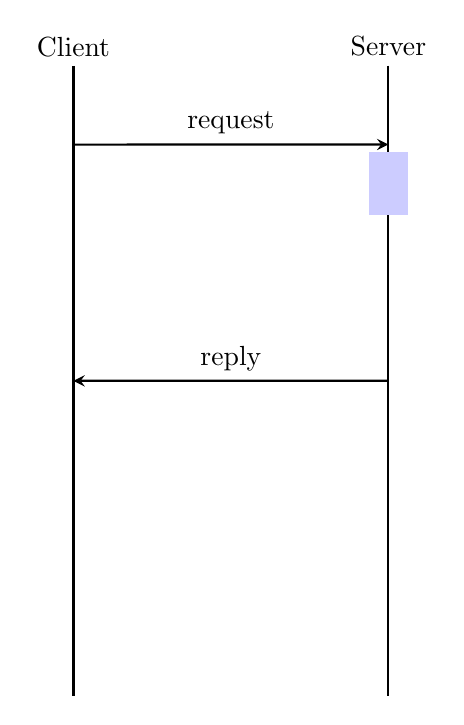
\begin{tikzpicture}[
    lifeline/.style={thick},
    message/.style={->, >=stealth, thick},
    activation/.style={rectangle, fill=blue!20, minimum width=0.5cm, minimum height=0.8cm} ]

    % Define lifelines
    \node[] (client) at (0,0) {Client};
    \node[] (server) at (4,0) {Server};
    % \node[] (database) at (8,0) {Database};

    % Draw lifelines
    \draw[lifeline] (client.south) -- ++(0,-8);
    \draw[lifeline] (server.south) -- ++(0,-8);
    % \draw[lifeline] (database.south) -- ++(0,-8);

    % Draw messages
    \draw[message] ([yshift=-1cm] client.south) -- node[above] {request} ([yshift=-1cm] server.south);
    % \draw[message] ([yshift=-2cm] server.south) -- node[above] {query} ([yshift=-2cm] database.south);
    % \draw[message] ([yshift=-3cm] database.south) -- node[above] {response} ([yshift=-3cm] server.south);
    \draw[message] ([yshift=-4cm] server.south) -- node[above] {reply} ([yshift=-4cm] client.south);

    % Draw activations
    \node[activation] at ([yshift=-1.5cm] server.south) {};
    % \node[activation] at ([yshift=-2.5cm] database.south) {};

    % Optional: Add dashed lines for return messages
    % \draw[dashed] ([yshift=-3cm] database.south) -- ++(0,-1);
    \draw[dashed] ([yshift=-4cm] server.south) -- ++(0,-1);

\end{tikzpicture}




waits for a sequences the packets in order (possibly wait
for out of order packets to arrive), processing them all together process all
the When the client has processed a batch of packets 

\section{Spec}
